\documentclass{report}
\usepackage[utf8]{inputenc}
\usepackage[francais]{babel}  
\usepackage[T1]{fontenc} 
\usepackage{graphicx}
\usepackage{listings}
\renewcommand{\thesection}{\arabic{section}}
\begin{document}
\title{%
    \begin{minipage}\linewidth
        \centering
        Projet Vega-Missyl
        \vskip 3pt
        \author{ Doha ROUIBAA & Pablo BOURDELAS & Guillaume RYCKAERT }
    \end{minipage}
    \begin{figure}[ht!]
        \centering
        \includegraphics[width=100mm]{bolideur.jpg}
    \end{figure}
}
\maketitle

\section*{Détermination des paramètres}

\subsection*{Tailles des données}
    \begin{figure}[ht!]
        \centering
        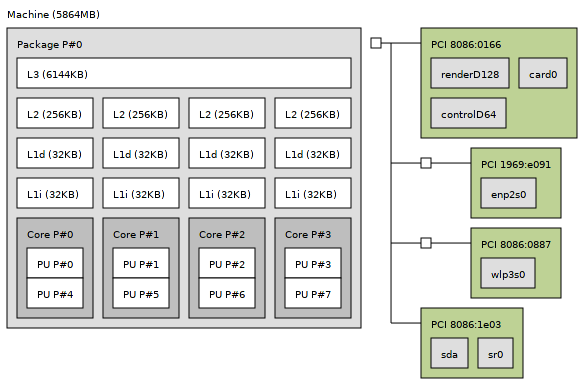
\includegraphics[width=100mm]{MEDIA/Topo.png}
        \caption{Caractéristiques de la machine utilisé}
    \end{figure}
\lstinputlisting{../kernel.c}

Notre boucle a besoin de 3 tableaux de taille n et d'un tableau de taille n$\times$n.\\
Chaque case du tableau prend 4 octets (int32\_t/float)\\
Le coût total en mêmoire est donc de $4n^2+12n$ octets.\\

Le cache L1 fait 32Ko, il faut donc prendre des tableaux de 85 cases. Coût total: 29.920 Ko

Le cache L2 fait 256Ko, il faut donc prendre des tableaux de 238 cases. Coût total: 229.432 Ko

Le cache L3 fait 6144Ko, il faut donc prendre des tableaux de 865 cases. Coût total: 3 003.280 Ko

Pour la RAM, nous prenons des tableaux de 2120 cases: coût total 18 003.04 Ko.

\begin{tabular}{ l c | c c }
    Type de Mémoire & Taille Mémoire & Taille Tableau & Coût Total\\\hline
    L1 & 32Ko & 85 & 29.920 Ko\\ 
    L2 & 256Ko & 238 & 229.432 Ko \\
    L3 & 6 144Ko & 865 & 3 033.280 Ko \\
    RAM & 5 864Mo & 2120 & 18.00304 Mo \\
\end{tabular}

\subsection*{Warmup}

Pour determiner le nombre de cycles de warmup nécessaires: On lance plusieurs fois la boucle de warmup, et l'on trace le graphe du temps d'éxécution en fonction du nombre de répétitons successives.

On sépare les cas pour les différent tailles de données:




-> méta-répétitions

->likwid(taille cache/tableaux)
->qualité code.





\end{document}
